% =====================================================================
\chapter{Methodology}
\label{ch:method}
% =====================================================================

This chapter describes the detector in full. It begins with the overall pipeline, then
covers the automatic generation of training labels, the canonical feature and the three
new internal-state features in self-contained notation, the wider feature families used
in the ablation, the classifier, the evaluation protocol, the baselines, and finally the
models and the free-hardware setup under which everything runs.

\section{Overall pipeline}

The detector reads signals from one forward pass of a frozen language model and feeds
them to a small classifier. Figure~\ref{fig:pipeline} shows the flow. A prompt --- during
training, a truncated encyclopedia article; during evaluation, a benchmark question or
document --- is given to the model, which generates a short continuation. From that single
pass we read four things: the canonical hidden state (the last-token vector at the final
layer), and three scalar summaries of the model's internal behaviour, namely how much its
representation drifts from layer to layer, how much it varies across layers, and how
uncertain it is while generating. These are concatenated into one feature vector and
passed to a five-layer perceptron that outputs a hallucination probability. The model
weights are never updated; only the small classifier is trained.

\begin{figure}[t]
\centering
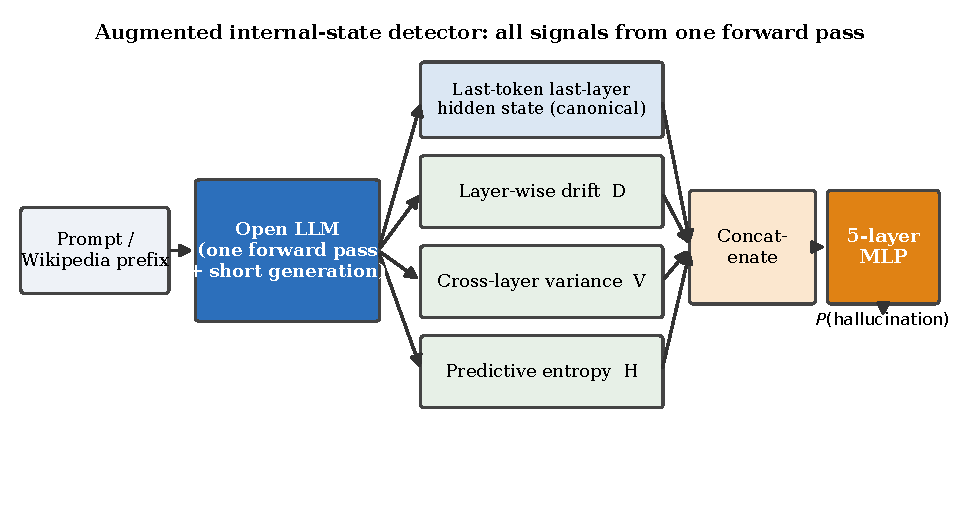
\includegraphics[width=0.99\textwidth]{images/ch04_methods/ch04_1_pipeline.pdf}
\caption{The augmented internal-state detector. Every signal is read from one forward
pass of a frozen model, so detection adds negligible cost over normal generation.}
\label{fig:pipeline}
\end{figure}

\section{Automatic label generation}
\label{sec:labels}

Supervised detection needs labelled examples, and labelling generations by hand does not
scale. We adopt the label-free procedure of the MIND framework~\cite{su2024mind},
illustrated in Figure~\ref{fig:pseudolabel} and stated as Algorithm~\ref{alg:label}. We
take an article, keep its first sentences, and find a named entity that occurs after the
first sentence. We truncate the text just before that entity and let the model predict
the continuation. If the entity the article actually had is among the model's top few
predicted first tokens, the model has stayed faithful, and we label the continuation
$y=0$. If the model instead produces a different entity, the continuation is factually
wrong with respect to the article; we let it generate on, then splice the article's
original suffix back so that the faithful and hallucinated versions differ only in the
entity span, and we label it $y=1$. The threshold for ``among the top few'' is the top
four predictions throughout.

\begin{figure}[h]
\centering
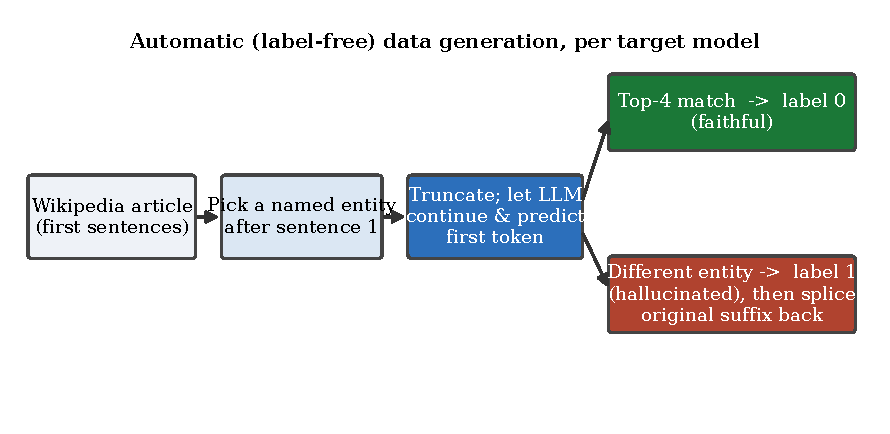
\includegraphics[width=0.96\textwidth]{images/ch04_methods/ch04_0_pseudolabel.pdf}
\caption{Automatic, label-free data generation. The model's own first-token prediction
decides the label; no human annotation is used, and the procedure is re-run separately
for each target model.}
\label{fig:pseudolabel}
\end{figure}

\begin{algorithm}[h]
\caption{Automatic label generation for one article}
\label{alg:label}
\begin{algbody}
\albf{Input:} article text, target model $M$, top-$k$ threshold $k=4$\\
\aln{1:}keep the first sentences; find a named entity $e$ occurring after sentence one\\
\aln{2:}truncate the text just before $e$ to form a prefix $x$\\
\aln{3:}let $M$ predict the next-token distribution given $x$\\
\aln{4:}\albf{if} $e$'s first token is among $M$'s top-$k$ predictions \albf{then}\\
\aln{5:}\alin label the continuation faithful ($y \gets 0$)\\
\aln{6:}\albf{else}\\
\aln{7:}\alin let $M$ generate until the original post-entity anchor reappears\\
\aln{8:}\alin splice the article's original suffix back onto the generated span\\
\aln{9:}\alin label the continuation hallucinated ($y \gets 1$)\\
\aln{10:}\albf{end if}\\
\aln{11:}\albf{return} labelled example $(x \,\Vert\, \text{continuation},\; y)$
\end{algbody}
\end{algorithm}

Two properties of this procedure matter. It produces balanced, per-model data at no
annotation cost, and --- because the prior literature shows probes do not transfer between
models --- it is run \emph{separately for each model} we study, so the training data always
comes from the same model the detector will monitor. For the larger models we generate one
thousand examples per class, two thousand in total.

\section{The canonical feature}

The backbone feature, which we call the \emph{canonical feature}, is the contextualised
vector at the last token of the final transformer layer~\cite{su2024mind}. Writing
$\zvec_\ell$ for the last-token activation at layer $\ell$ and $L$ for the number of
layers, the canonical feature is simply $\hvec = \zvec_L$. Its dimension equals the
model's hidden width $d$ --- for the six-billion-parameter model that anchors our results,
$d=4096$. Every configuration in the ablation includes this feature; the question the
ablation answers is what, if anything, the additional scalars buy on top of it.

\section{Three internal-state features}
\label{sec:trio}

The core proposal of this dissertation is to summarise the model's internal behaviour
during a generation with three inexpensive scalars, all computed from activations that
the forward pass already produced. We use fresh notation throughout: $\zvec_\ell$ is the
last-token activation vector at layer $\ell$, and $p_t(\cdot)$ is the model's token
distribution at generation step $t$.

\paragraph{Layer-wise representation drift.}
As information moves up the layer stack, the representation of a token changes. We measure
how much by the cosine distance between adjacent layers,
\begin{equation}
d_\ell \;=\; 1 - \frac{\zvec_\ell \cdot \zvec_{\ell+1}}{\lVert \zvec_\ell\rVert\,\lVert \zvec_{\ell+1}\rVert},
\qquad \ell = 1,\dots,L-1,
\end{equation}
and summarise the whole trajectory by its mean,
\begin{equation}
\Dmean \;=\; \frac{1}{L-1}\sum_{\ell=1}^{L-1} d_\ell .
\end{equation}
A faithful continuation tends to settle into a stable trajectory; large or erratic drift
is a candidate signal of trouble.

\paragraph{Cross-layer variance.}
A complementary view asks how spread out the layer representations are around their own
average. With the layer-wise mean $\bar{\zvec} = \tfrac{1}{L}\sum_{\ell=1}^{L}\zvec_\ell$,
we define
\begin{equation}
\Vlast \;=\; \frac{1}{L}\sum_{\ell=1}^{L}\bigl\lVert \zvec_\ell - \bar{\zvec}\bigr\rVert_2^{2}.
\end{equation}
Whereas drift is a sequential, layer-to-layer quantity, the variance is a global measure
of dispersion across the whole stack. Only the scalar $\Vlast$ is stored; the mean
$\bar{\zvec}$ is internal to its computation.

\paragraph{Predictive entropy.}
The third scalar looks at the output distribution rather than the hidden states. At each
generation step the Shannon entropy of the token distribution is
\begin{equation}
H^{(t)} \;=\; -\sum_{w \in V} p_t(w)\,\log p_t(w),
\end{equation}
where $V$ is the vocabulary, and we average it over the $T$ generated steps,
\begin{equation}
\Hmean \;=\; \frac{1}{T}\sum_{t=1}^{T} H^{(t)} .
\end{equation}
High predictive entropy means the model was unsure as it generated, which is weak but
useful evidence of hallucination.

The three scalars $\{\Dmean,\Vlast,\Hmean\}$ are concatenated onto the canonical feature.
Crucially, all three are intra-sample summaries from a single pass: they involve no extra
sampling, no auxiliary model, and no optimal-transport computation, which keeps them
clearly distinct from the prior study discussed in Section~\ref{sec:internal} and keeps
their cost negligible.

\section{Two wider feature families}

To place the three core features in context, the ablation also includes two further
families of scalar features, all read from the same single pass.

\paragraph{Literature features.}
A set of nine scalars is drawn from recent internal-state work. They include a
\emph{lookback ratio} that compares attention paid to the context against attention paid
to freshly generated tokens~\cite{chuang2024lookback}; an \emph{attention-sink} score
that measures how much attention mass collapses onto the first
token~\cite{xiao2023streamingllm}; a lightweight eigenvalue-based dispersion of the hidden
states in the spirit of the INSIDE method~\cite{chen2024inside}; an internal-consistency
ratio; a \emph{logit-lens divergence}, the Jensen--Shannon divergence (abbreviated JSD: a
symmetric measure of how different two probability distributions are) between the
vocabulary distributions read off from an early and a late layer, following the
contrast-between-layers idea~\cite{chuang2024dola}; an attention-head entropy; a
token-level confidence margin in the spirit of adaptive token-selection
work~\cite{niu2025hami}; the rank of the chosen token in the output distribution; and a
within-layer dispersion of token embeddings in the spirit of reasoning-aware
detection~\cite{d2hscore2025}. A tenth, supervised mid-layer probe feature is left for
future work because it would require training a separate probe inside the pipeline; we
note its omission rather than quietly dropping it.

\paragraph{Exploratory features.}
A second set of six scalars is more speculative and is included to test whether less
conventional signals help. In reader-facing terms these are: a small projection of the
hidden state through the model's output vocabulary head; a measure of the curvature of the
layer trajectory; the slope and variance of the model's confidence over the course of the
generation; an effective rank of the attention matrix; an alignment score between the
generated text and the prompt; and a divergence of the per-head importance distribution.
These are reported for completeness; we do not lean on them for any central claim.

\section{Feature configurations}
\label{sec:configs}

The ablation evaluates sixteen configurations, each being the canonical feature plus a
chosen subset of scalar features, as laid out in Figure~\ref{fig:families} and
Table~\ref{tab:configs}. The configurations move from the canonical feature alone, through
each new scalar added singly, to the three-scalar internal-state set, to the literature
set, to the exploratory set, and finally to combinations of these. Throughout the
dissertation we refer to configurations by a neutral index and a short description; we do
not use the working code names from the implementation. The configuration consisting of
the canonical feature plus the three internal-state scalars (configuration~5) is the
headline proposal, and we call it the \emph{augmented internal-state detector}.

\begin{figure}[t]
\centering
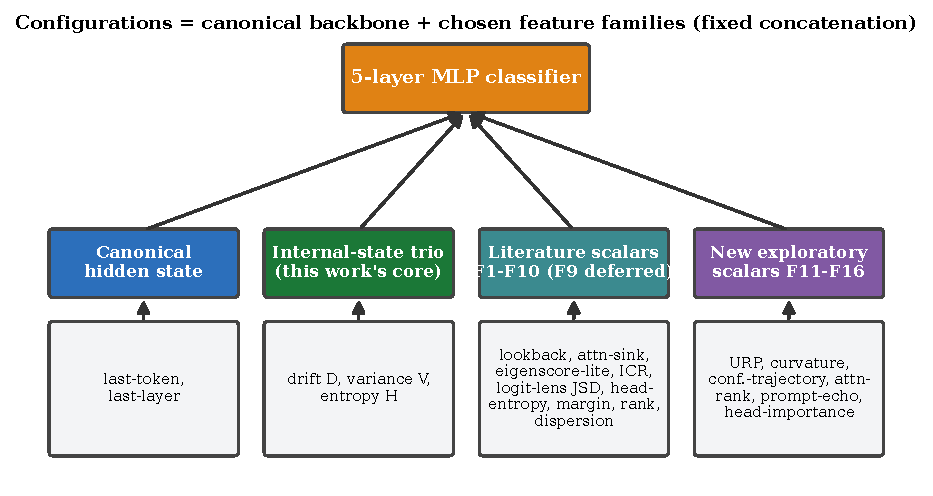
\includegraphics[width=0.97\textwidth]{images/ch04_methods/ch04_2_feature_families.pdf}
\caption{The feature families that make up the configurations. Each configuration is the
canonical backbone plus a fixed concatenation of chosen scalar families; there is no
automatic feature selection.}
\label{fig:families}
\end{figure}

\begin{table}[t]
\centering
\caption{The sixteen feature configurations. The input dimension is shown for the
six-billion-parameter model (hidden width $d=4096$); for other models the canonical part
changes with $d$ while the scalar counts stay the same.}
\label{tab:configs}
\small
\renewcommand{\arraystretch}{1.15}
\begin{tabular}{cl c c}
\toprule
\textbf{Cfg.} & \textbf{Feature content} & \textbf{\# scalars} & \textbf{MLP input dim} \\
\midrule
C1  & Canonical feature only (backbone)                         & 0  & 4096 \\
C2  & Canonical + drift                                         & 1  & 4097 \\
C3  & Canonical + cross-layer variance                          & 1  & 4097 \\
C4  & Canonical + predictive entropy                            & 1  & 4097 \\
C5  & Canonical + internal-state trio (\emph{this work})        & 3  & 4099 \\
C6  & Canonical + lookback ratio                                & 1  & 4097 \\
C7  & Canonical + logit-lens divergence                         & 1  & 4097 \\
C8  & Canonical + confidence margin                             & 1  & 4097 \\
C9  & Canonical + lookback/lens/margin trio                     & 3  & 4099 \\
C10 & Canonical + all nine literature features                  & 9  & 4105 \\
C11 & Canonical + internal-state trio + lookback/lens/margin     & 6  & 4102 \\
C12 & Canonical + internal-state trio + all literature           & 12 & 4108 \\
C13 & Canonical + vocab projection + curvature                  & 10 & 4106 \\
C14 & Canonical + confidence-trajectory/rank/echo               & 4  & 4100 \\
C15 & Canonical + vocab projection/curvature/confidence         & 12 & 4108 \\
C16 & Canonical + internal-state trio + all exploratory          & 18 & 4114 \\
\bottomrule
\end{tabular}
\end{table}

\section{The classifier}

Every configuration uses the same classifier, so that differences in measured performance
come from the features and not from the model on top of them. The classifier is a
five-layer perceptron with progressively narrowing hidden widths and rectified-linear
activations, ending in a two-way softmax that outputs the probability of each class. It is
trained with the cross-entropy loss using the Adam optimiser at a learning rate of
$5\times10^{-4}$ and weight decay $10^{-5}$, with a batch size of $32$, for ten epochs.
The scalar and canonical features are standardised by a scaler fitted on the training
split only, and the data is split $80/20$ into training and test sets with a fixed random
seed of $42$ so that every configuration sees exactly the same partition. The use of a
fixed, five-layer perceptron with cross-entropy and no feature selection is a deliberate
design commitment that distinguishes this work from the multi-feature, metric-learning
prior study of Section~\ref{sec:internal}.

\section{Evaluation protocol}
\label{sec:protocol}

After training on the encyclopedia-continuation data, each detector is evaluated in two
regimes. The \emph{in-distribution} regime uses a held-out split of the same
encyclopedia-continuation data. The \emph{transfer} regime uses a multi-benchmark suite
of question-answering, summarisation, and dialogue tasks that the detector never saw
during training. Algorithm~\ref{alg:eval} states the protocol.

To make the comparison fair and cheap, every method --- configuration or baseline --- is
scored on the \emph{same} fixed set of rows from each benchmark: a deterministic first-$N$
slice, with $N$ up to $350$ rows per benchmark in the fully unified runs. Because both the
configuration runs and the baseline runs read the same rows, their scores are directly
comparable. The transfer suite contains up to ten benchmarks: the four
question-answering sets TruthfulQA~\cite{lin2022truthfulqa},
TriviaQA~\cite{joshi2017triviaqa}, CoQA~\cite{reddy2019coqa} and
TyDi~QA~\cite{clark2020tydiqa}; the three directly labelled HaluEval
subsets~\cite{li2023halueval}; and three further question-answering sets, Natural
Questions~\cite{kwiatkowski2019nq}, HotpotQA~\cite{yang2018hotpotqa} and
PopQA~\cite{mallen2023popqa}. Each benchmark is wrapped in a short, fixed instruction
prompt appropriate to its task; the prompt wording is held constant across all methods.

\begin{algorithm}[h]
\caption{Single-pass feature extraction and multi-task evaluation}
\label{alg:eval}
\begin{algbody}
\albf{Input:} trained classifier $C$, target model $M$, benchmark suite $\mathcal{D}$, slice size $N$\\
\aln{1:}\albf{for} each benchmark $D \in \mathcal{D}$ \albf{do}\\
\aln{2:}\alin \albf{for} each of the first $N$ rows of $D$ \albf{do}\\
\aln{3:}\alinn run $M$ once on the prompt; collect last-layer hidden state and per-layer activations\\
\aln{4:}\alinn compute the canonical feature and the chosen scalars (drift, variance, entropy, \dots)\\
\aln{5:}\alinn standardise with the training scaler; obtain $\hat{p}=C(\mathbf{x})$\\
\aln{6:}\alin \albf{end for}\\
\aln{7:}\alin compute AUROC, accuracy, precision, recall, F1 (and calibration where available)\\
\aln{8:}\albf{end for}\\
\aln{9:}\albf{return} per-benchmark metrics and their mean
\end{algbody}
\end{algorithm}

\section{Baselines}
\label{sec:baselines}

The detectors are compared against four established methods plus two simple reference
methods, all re-implemented inside the same pipeline and scored on the same rows.
Table~\ref{tab:baselines} summarises them. SAPLMA~\cite{azaria2023saplma} is a supervised
probe on a single intermediate layer's hidden state. HaloScope~\cite{du2024haloscope} is
the unsupervised spectral method that estimates pseudo-labels from a latent subspace.
HalluShift~\cite{dasgupta2025hallushift} is the multi-feature supervised method of
Section~\ref{sec:internal}, re-implemented from its description with a thirty-one
dimensional feature vector. EigenScore is the sampling-based covariance score from the
INSIDE method~\cite{chen2024inside}. To these we add two reference points: MIND, a
supervised probe on the final-layer hidden state --- effectively the method this work
extends~\cite{su2024mind} --- and Perplexity, an unsupervised score equal to the mean
token negative log-likelihood (abbreviated NLL), where a higher value of the continuation's
perplexity is taken as weak evidence of hallucination.

Two further methods were considered as baselines and deliberately left out of the final
set. Semantic entropy~\cite{kuhn2023semantic} requires drawing several samples per prompt
and loading an auxiliary natural-language-inference model, which adds several hours of
computation per large model and would have broken the free-tier time budget. The
attention-only Lookback Lens~\cite{chuang2024lookback} was dropped because the attention
statistics it relies on are already represented among our features and among HalluShift's,
so it added a row without adding a new paradigm. The final baseline set is therefore the
four established methods plus the two reference scores.

\begin{table}[t]
\centering
\caption{Baselines re-implemented inside the unified pipeline. ``Dim'' is the
dimensionality of each method's feature or score for the six-billion-parameter model.}
\label{tab:baselines}
\small
\renewcommand{\arraystretch}{1.2}
\begin{tabularx}{\textwidth}{l l c X}
\toprule
\textbf{Baseline} & \textbf{Paradigm} & \textbf{Dim} & \textbf{Signal} \\
\midrule
SAPLMA      & supervised probe          & 4096 & hidden state at a single intermediate layer \\
HaloScope   & unsupervised spectral     & 4096 & best-layer hidden, pseudo-labelled from a subspace \\
HalluShift  & supervised multi-feature  & 31   & layer distribution-shift + attention + probability features \\
EigenScore  & sampling-based (score)    & 1    & log-determinant of the covariance of several samples \\
MIND        & supervised probe          & 4096 & final-layer last-token hidden state \\
Perplexity  & unsupervised (score)      & 1    & mean token negative log-likelihood \\
\bottomrule
\end{tabularx}
\end{table}

\section{Models and free-hardware implementation}
\label{sec:models}

A goal of this dissertation is that every experiment runs on free cloud hardware, so that
the study can be reproduced without a research budget. The primary platform is a free
Kaggle notebook with two T4 GPUs of sixteen gigabytes each, giving thirty-two gigabytes of
combined video memory (abbreviated VRAM) through model parallelism, used in the bfloat16
sixteen-bit number format (abbreviated bf16) with no further quantisation. Sessions are
capped at nine hours, within a weekly budget of thirty GPU-hours. A free Colab notebook
with a single T4 serves as a fallback for the smaller models. The seven-billion-parameter
models require both T4 GPUs; a single sixteen-gigabyte card cannot hold a seven-billion
model in bf16 together with the memory needed for generation.

Table~\ref{tab:models} lists the models. The fleet spans a tiny diagnostic model used only
to verify pipeline correctness, two sub-one-billion and one-to-three-billion models for
fast iteration, and a set of six- to seven-billion models that constitute the substantive
study. The six-billion-parameter model is the one for which a complete set of
configuration and baseline measurements exists, and it anchors the results of
Chapter~\ref{ch:results}.

\begin{table}[t]
\centering
\caption{Models in the study. ``Role'' distinguishes the substantive models from the small
models used for iteration and the tiny model used only as a correctness check. Hidden
width and layer count are listed where they anchor later results.}
\label{tab:models}
\small
\renewcommand{\arraystretch}{1.2}
\begin{tabular}{l c c l}
\toprule
\textbf{Model} & \textbf{Parameters} & \textbf{Hidden / layers} & \textbf{Role} \\
\midrule
GPT-J~\cite{wang2021gptj}            & 6.0\,B  & 4096 / 28 & substantive (complete measurements) \\
OPT~\cite{zhang2022opt}              & 6.7\,B  & 4096 / 32 & substantive \\
Llama-2~\cite{touvron2023llama2}     & 7\,B    & ---        & substantive (gated; data limited) \\
Mistral~\cite{jiang2023mistral}      & 7\,B    & ---        & substantive (results pending) \\
Falcon~\cite{almazrouei2023falcon}   & 7\,B    & ---        & substantive (results pending) \\
Qwen2.5~\cite{qwen2024report}        & 3\,B    & 2560 / --- & iteration / in-distribution \\
TinyLlama~\cite{zhang2024tinyllama}  & 1.1\,B  & 2048 / --- & iteration / in-distribution \\
Qwen2.5 (small)~\cite{qwen2024report}& 0.5\,B  & ---        & fast iteration \\
GPT-2~\cite{radford2019gpt2}         & 0.12\,B & ---        & smoke test (diagnostic only) \\
\bottomrule
\end{tabular}
\end{table}

In summary, the methodology fixes everything except the features: the same automatic
labels, the same classifier, the same split and seed, the same evaluation rows, and the
same hardware regime. This is what makes the comparison in the next chapter a comparison
of \emph{features}, and what makes it reproducible on a free account.
